\section{Experiments}

\subsection{In-Sample}

We evaluated whether the DQN could overfit small datasets and outperform \texttt{-Oz}. For these experiments, we used the change in instruction count as the 
reward, Autophase features for the program representation, and applied online standardization to rewards and features. As shown in 
Figure~\ref{fig:in_sample_qsort}, the DQN was able to outperform \texttt{-Oz} in-sample.
% and Figure~\ref{fig:in_sample_tensorflow}

\begin{figure}[h]
    \centering
    \label{fig:in_sample_qsort}
    \includegraphics[scale=0.5]{in_sample_qsort.png}
    \caption{In-sample performance on a quicksort function.}
\end{figure}

% \begin{figure}
%     \centering
%     \label{fig:in_sample_tensorflow}
%     \includegraphics[scale=0.5]{in_sample_tensorflow.png}
%     \caption{In-sample performance on Tensorflow~\cite{abadi2016} objects.}
% \end{figure}

\subsection{Hyperparameter Sweep}

\begin{table}[h]
    \label{tab:hyperparameters}
    \caption{Hyperparameter Sweep}
    \centering
    \begin{tabular}{ll}
    \toprule
    \textbf{Hyperparameter} & \textbf{Value(s)} \\
    \midrule
    Signed Reward & Yes, No \\
    Autoencoder & Yes, No \\
    DQN Hidden Size & 256, 512 \\
    Learning Rate & 0.0005, 0.00005 \\
    \bottomrule
    \end{tabular}
\end{table}

We conducted a hyperparameter sweep to determine the best combination of rewards and feature representation. See 
Table~\ref{tab:hyperparameters} for combinations. All combinations used an initial epsilon-greedy probability of 90\% linearly decayed to 1\% over 32,768 steps, 
were trained on the AnghaBench dataset, used 64 steps per episode for 1,024 episodes with a batch size of 128 and 32 batches per episode. The memory capacity was set at 8,192
entries and filled to 50\% before training began. Detailed results are provided in Figure~\ref{fig:sweep}. Notably, signed rewards stabilized the training 
procedure while the autoencoder did not.

\begin{figure}[h]
    \centering
    \label{fig:sweep}
    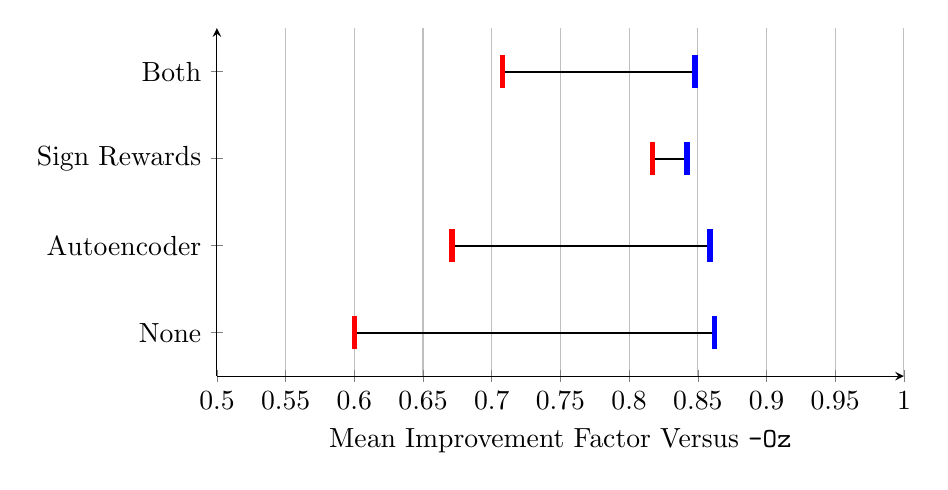
\begin{tikzpicture}
    \begin{axis}[
        xmajorgrids,
        xlabel={Mean Improvement Factor Versus \texttt{-Oz}},
        ytick={1,2,3,4},
        yticklabels={None, Autoencoder, Sign Rewards, Both},
        width=0.85\columnwidth,
        height=6cm,
        xmin=0.5,
        xmax=1,
        ymin=0.5,
        ymax=4.5,
        enlarge y limits=0.15,
        axis y line=left,
        axis x line=bottom,
    ]

    \addplot+[thick, black, mark=none, line cap=round] coordinates { (0.600,1) (0.862,1) } node[right,pos=0.95] {}; 
    \addplot+[thick, black, mark=none, line cap=round] coordinates { (0.671,2) (0.859,2) } node[right,pos=0.95] {};
    \addplot+[thick, black, mark=none, line cap=round] coordinates { (0.817,3) (0.842,3) } node[right,pos=0.95] {};
    \addplot+[thick, black, mark=none, line cap=round] coordinates { (0.708,4) (0.848,4) } node[right,pos=0.95] {};

    \addplot+[
        only marks,
        mark=|,
        mark size=6pt,
        mark options={line width=2pt, solid, red}
        ] coordinates { (0.600,1) (0.671,2) (0.817,3) (0.708,4) };
    \addplot+[only marks, mark=|, mark size=6pt, mark options={line width=2pt, solid}, blue] coordinates { (0.862,1) (0.859,2) (0.842,3) (0.848,4) };

    \end{axis}
    \end{tikzpicture}
    \caption{Geometric mean improvement factor versus \texttt{-Oz} across six benchmark suites. Blue (red) line is maximum (minimum) improvement factor in hyperparameter sweep.}
\end{figure}

\subsection{Final Model}

\begin{figure*}[t!]
    \centering
    \label{fig:results}
    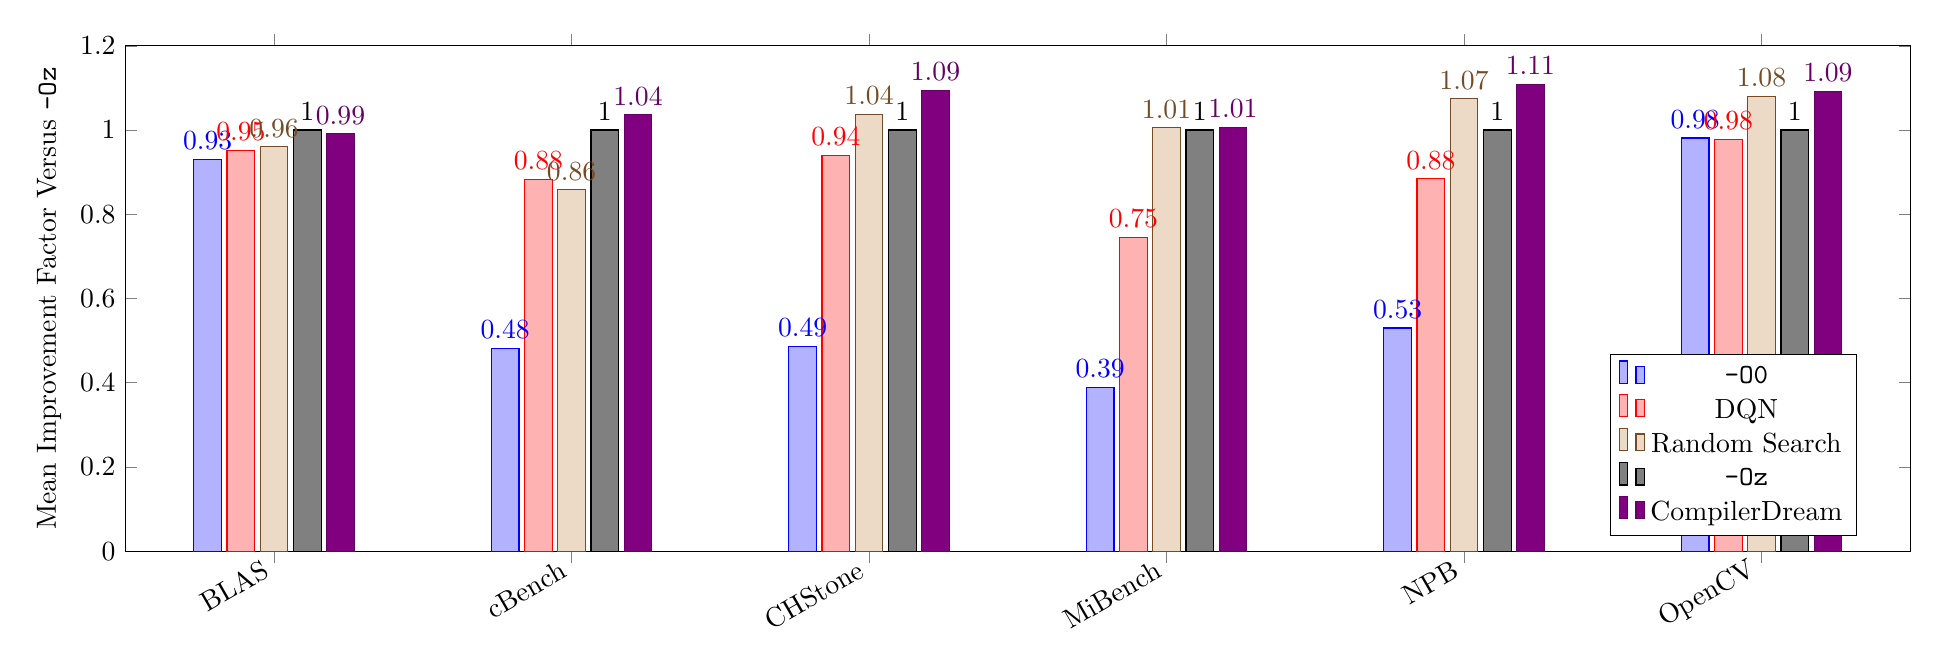
\begin{tikzpicture}
    \begin{axis}[
        ybar,
        bar width=10pt,
        width=2*\columnwidth,
        height=8cm,
        ylabel={Mean Improvement Factor Versus \texttt{-Oz}},
        symbolic x coords={BLAS,cBench,CHStone,MiBench,NPB,OpenCV},
        xtick=data,
        ymin=0,
        ymax=1.2,
        legend style={
            anchor=south east,
            at={(0.97, 0.03)},
            % legend columns=3
        },
        nodes near coords,
        nodes near coords align={vertical},
        x tick label style={rotate=30, anchor=east}
    ]

    % -O0
    \addplot coordinates {
        (BLAS,0.931)
        (cBench,0.481)
        (CHStone,0.487)
        (MiBench,0.389)
        (NPB,0.530)
        (OpenCV,0.981)
    };

    % Mine
    \addplot coordinates {
        (BLAS,0.951)
        (cBench,0.883)
        (CHStone,0.940)
        (MiBench,0.745)
        (NPB,0.884)
        (OpenCV,0.978)
    };

    % Random Search
    \addplot coordinates {
        (BLAS,0.960)
        (cBench,0.858)
        (CHStone,1.037)
        (MiBench,1.005)
        (NPB,1.074)
        (OpenCV,1.080)
    };

    % -Oz
    \addplot coordinates {
        (BLAS,1.000)
        (cBench,1.000)
        (CHStone,1.000)
        (MiBench,1.000)
        (NPB,1.000)
        (OpenCV,1.000)
    };

    % CompilerDream
    \addplot coordinates {
        (BLAS,0.991)
        (cBench,1.036)
        (CHStone,1.094)
        (MiBench,1.006)
        (NPB,1.108)
        (OpenCV,1.092)
    };

    \legend{\texttt{-O0}, DQN, Random Search, \texttt{-Oz}, CompilerDream}

    \end{axis}
    \end{tikzpicture}
    \caption{DQN geometric mean IR instruction count reduction over \texttt{-Oz} on six representative benchmark suites. See Table~\ref{tab:datasets} for 
    additional details.}
\end{figure*}

We selected the hyperparameter combination with maximum speedup on the training set and trained it on AnghaBench for one day with 64 steps per episode. This
combination used an autoencoder with the IR instruction count change reward. Due to time constraints, we could not wait for test metrics to become available. 
We also attempted curriculum learning, training the final model for another day with 256 steps per episode. We evaluated both the final model and the final 
model with curriculum learning at 64 and 256 steps for episode. Only the final model with 64 step per episode had reasonable performance, attaining 89\% of the
IR instruction count reduction obtained by \texttt{-Oz}. The full results are available in Figure~\ref{fig:results}.

\begin{table}
    \caption{Training and Evaluation Datasets}
    \label{tab:datasets}
    \centering
    \renewcommand{\arraystretch}{1.15}
    \begin{tabular}{
        p{2.0cm}
        p{1.0cm}
        p{4.0cm}
    }
        \toprule
        \textbf{Dataset} &
        \textbf{Samples} &
        \textbf{Description} \\
        \midrule
        AnghaBench~\cite{dasilva2021} & 1,041,333 & C/C++ functions extracted from GitHub \\
        BLAS~\cite{blas2002} & 300 & Linear algebra kernels \\
        cBench~\cite{fursin2014} & 23 & C benchmarks \\
        CHStone~\cite{hara2008} & 12 & C-based high-level synthesis benchmarks \\
        MiBench~\cite{guthaus2001} & 40 & Embedded C benchmarks \\
        NPB & 122 & NASA parallel benchmarks \\
        OpenCV~\cite{culjak2012} & 442 & C++ objects from OpenCV \\
        \bottomrule
    \end{tabular}
\end{table}
